\documentclass[
	% -- opções da classe memoir --
	12pt,				% tamanho da fonte
	% openright,			% capítulos começam em pág ímpar (insere página vazia caso preciso)
	oneside,			% para impressão em recto e verso. Oposto a oneside
	a4paper,			% tamanho do papel.
	% -- opções da classe abntex2 --
  section=TITLE,
  % subsection=TITLE,
	% chapter=TITLE,		% títulos de seções convertidos em letras maiúsculas
  % section=TITLE,
	%subchapter=TITLE,	% títulos de subseções convertidos em letras maiúsculas
	%subsubchapter=TITLE,% títulos de subsubseções convertidos em letras maiúsculas
	% -- opções do pacote babel --
  % sumario=tradicional
	brazil,				% o último idioma é o principal do documento
	]{abntex2}

% ---
% PACOTES
% ---

% ---
% Pacotes fundamentais
% ---
% Fonte ARIAL
\usepackage{helvet}
\renewcommand{\familydefault}{\sfdefault}
%------
% \usepackage{lmodern}			% Usa a fonte Latin Modern
\usepackage[T1]{fontenc}		% Selecao de codigos de fonte.
\usepackage[utf8]{inputenc}		% Codificacao do documento (conversão automática dos acentos)
\usepackage{indentfirst}		% Indenta o primeiro parágrafo de cada seção.
\usepackage{color}				% Controle das cores
\usepackage{graphicx}			% Inclusão de gráficos
\usepackage{microtype} 			% para melhorias de justificação
% ---

%Para links
\usepackage{hyperref}
% ---
% Pacotes adicionais, usados apenas no âmbito do Modelo Canônico do abnteX2
% ---
\usepackage{lipsum}				% para geração de dummy text
% ---

% ---
% Pacotes de citações
% ---
\usepackage[brazilian,hyperpageref]{backref}	 % Paginas com as citações na bibl
\usepackage[alf]{abntex2cite}	% Citações padrão ABNT

% ---
% CONFIGURAÇÕES DE PACOTES
% ---

%% Estilizando section
\usepackage{titlesec}
\titleformat{\section}    {\normalfont\fontfamily{phv}\fontsize{12}{17}\bfseries}{\thesection}{1em}{}
\renewcommand{\ABNTEXsectionfontsize}{\normalsize}
\titleformat{\subsection}    {\normalfont\fontfamily{phv}\fontsize{12}{17}\bfseries}{\thesubsection}{1em}{}
\renewcommand{\ABNTEXsectionfontsize}{\normalsize}
%----

% ---
% Configurações do pacote backref
% Usado sem a opção hyperpageref de backref
\renewcommand{\backrefpagesname}{Citado na(s) página(s):~}
% Texto padrão antes do número das páginas
\renewcommand{\backref}{}
% Define os textos da citação
\renewcommand*{\backrefalt}[4]{
	\ifcase #1 %
		% Nenhuma citação no texto.%
	\or
		% Citado na página #2.%
	\else
		% Citado #1 vezes nas páginas #2.%
	\fi}%
% ---

  % opção para Artigo
\counterwithout{section}{section}
\counterwithout{figure}{chapter}
\counterwithout{table}{chapter}
\renewcommand{\footnotesize}{\small}



% ---
% Informações de dados para CAPA e FOLHA DE ROSTO
% ---
\titulo{Projeto Integrado Multidisciplinar IV}
\autor{ UNIP EaD\\
Andreia Domingues da Silva RA: 2023727\\
Bruna Rossanesi RA: 2016910\\
Douglas Pinheiro RA: 2014309\\
Mayara Verônica Oliveira Silva RA: 1889899\\
Natalia Fabricio Costa RA: 2006807\\
Pedro Expedito De Oliveira RA: 2028118}
\local{Santa Fé-PR}
\data{2020}
\instituicao{%
  Universidade Paulista -- Unip
  \par
  Faculdade de Analise e Desenvolvimento Sistemas
  \par
  Projeto Integrado Multidisciplinar}
\tipotrabalho{Tese (Doutorado)}
% O preambulo deve conter o tipo do trabalho, o objetivo,
% o nome da instituição e a área de concentração
\preambulo{Projeto Integrado Multidisciplinar para obtenção do título de tecnólogo
em Análise e Desenvolvimento de Sistemas apresentado à Universidade Paulista – UNIP EaD.\\
Orientador(a): Ellen Cristina Dias.}
% ---

% ---
% Configurações de aparência do PDF final

% alterando o aspecto da cor azul
\definecolor{blue}{RGB}{41,5,195}

% informações do PDF
\makeatletter
\hypersetup{
     	%pagebackref=true,
		pdftitle={\@title},
		pdfauthor={\@author},
    	pdfsubject={\imprimirpreambulo},
	    pdfcreator={LaTeX with abnTeX2},
		pdfkeywords={abnt}{latex}{abntex}{abntex2}{PIM},
		colorlinks=true,       		% false: boxed links; true: colored links
    	linkcolor=blue,          	% color of internal links
    	citecolor=blue,        		% color of links to bibliography
    	filecolor=magenta,      		% color of file links
		urlcolor=blue,
		bookmarksdepth=4
}
\makeatother
% ---

% ---
% Espaçamentos entre linhas e parágrafos
% ---

% O tamanho do parágrafo é dado por:
\setlength{\parindent}{1.3cm}

% Controle do espaçamento entre um parágrafo e outro:
\setlength{\parskip}{0.2cm}  % tente também \onelineskip

% ---
% compila o indice
% ---
% \makeindex
% ---

% ----
% Início do documento
% ----
\setlength\afterchapskip{\lineskip}
\begin{document}


% Seleciona o idioma do documento (conforme pacotes do babel)
\selectlanguage{brazil}

% Retira espaço extra obsoleto entre as frases.
\frenchspacing

% ----------------------------------------------------------
% ELEMENTOS PRÉ-TEXTUAIS
% ----------------------------------------------------------
% \pretextual

% ---
% Capa
% ---
\imprimircapa
% ---

% ---
% Folha de rosto
% ---
\imprimirfolhaderosto
% ---

% ---
% NOTA DA ABNT NBR 15287:2011, p. 4:
%  ``Se exigido pela entidade, apresentar os dados curriculares do autor em
%     folha ou página distinta após a folha de rosto.''
% ---

% ---
% inserir lista de ilustrações
% ---
% \pdfbookmark[0]{\listfigurename}{lof}
% \listoffigures*
% \cleardoublepage
% ---

% ---
% inserir lista de tabelas
% ---
% \pdfbookmark[0]{\listtablename}{lot}
% \listoftables*
% \cleardoublepage
% % ---

% ---
% inserir lista de abreviaturas e siglas
% ---
% \begin{siglas} \item[ABNT] Associação Brasileira de Normas Técnicas
% \item[abnTeX] ABsurdas Normas para TeX
% \end{siglas}
% ---

% ---
% inserir lista de símbolos
% ---
% \begin{simbolos}
%   \item[$ \Gamma $] Letra grega Gama
%   \item[$ \Lambda $] Lambda
%   \item[$ \zeta $] Letra grega minúscula zeta
%   \item[$ \in $] Pertence
% \end{simbolos}
% ---


\begin{resumo}

Este projeto integrado Multidicisplinar V, do Curso analise e desenvolvimento
de sistemas tem o objetivo de desenvolver um software de alta qualidade e
simplificando o armazenamento de dados de cada paciente, gerando um arquivo de
texto para salvar as informações referentes aos pacientes e a lista dos
pacientes no  grupo de risco que será enviada para secretaria da Saúde.
Contendo apenas as informações de CEP e Idade do paciente, mantendo em sigilo
todas as outras informações e seguindo a risca todos os requisitos e
funcionalidades apontadas no manual fornecido pela instituição UNIP.  Sendo o
projeto inteiramente desenvolvido em Linguagem C com a utilização apenas de
ferramentas livres como GIT, Neovim,  Mingw e GNU Debugger sendo indispensáveis
para realização do projeto.Vale destacar o Mingw como principal ferramenta
capaz de compilar Linguagem C para código de máquina que pode executar no
sistema operacional Windows da Microsoft que não oferece ferramenta livres para
desenvolver em sua própria plataforma, deixando o desenvolvedor dependente de
suas ferramentas e cerceando a sua liberdade.  Utilizando estas ferramentas é
possível ter uma melhor qualidade final no produto e mantendo os direitos sobre
o sistema desenvolvido e acima de tudo a liberdade.

 \textbf{Palavras-chave}: Covid-19, Linguagem C, hospitais.
\end{resumo}


% resumo em inglês
\begin{resumo}[Abstract]
 \begin{otherlanguage*}{english}
This integrated project Multidicisplinar V, of the course analyze and develop
systems has the objective of developing high quality software and simplifying
the data storage of each patient, generating a text file to save as information
related to patients and the list of patients in the risk group that will be
sent to the Secretary of Health. Containing only the information of the
patient's CEP and Age, keeping all information confidential and strictly
following all the requirements and characteristics indicated in the manual
provided by the UNIP institution. Being the developed project developed in
Language C using only free tools such as GIT, Neovim, Mingw and GNU Debugger
being indispensable for the realization of the project. Mingw stands out as the
main tool capable of compiling Language C for machine code that can run on
Microsoft's Windows operating system that doesn't offer free tools to develop
on its own platform, leaving the developer dependent on his tools and
curtailing his freedom. Using these tools it is possible to have a better final
quality in the product and keep the rights on the developed system and above
all freedom.\\
\\
   \vspace{\onelineskip}
   \noindent
   \textbf{Keywords}: Covid-19, C lang , Hospital.
 \end{otherlanguage*}
\end{resumo}


% ---
% inserir o sumario
% ---
\pdfbookmark[0]{\contentsname}{toc}
\tableofcontents*
\cleardoublepage
% ---
% ----------------------------------------------------------
% ELEMENTOS TEXTUAIS
% ----------------------------------------------------------
\textual

%Remover sumario do cabeçalho

\pagestyle{simple}
\aliaspagestyle{chapter}{simple}

% altera o espaçamento depois do número de cada secao, subsecao, etc.
%altera tamanho de fonte, negrito, itálico, etc.

% -------

% ----------------------------------------------------------
% Introdução
% ----------------------------------------------------------
\section{INTRODUÇÃO}
Com o grande crescimento de casos de corona vírus houve a necessidade de
softwares capazes de contribuir com a administração dos casos, ou seja um
software capaz de facilitar os cadastros economizando tempo dos profissionais
de saúde e com a finalidade de manter um acompanhamento progressivo para
inclusive , auxiliar nas tomadas de decisões e ações preventivas.

E para atender as necessidades dos profissionais de saúde em poder cadastrar
novos portadores do vírus COVID-19, o presente projeto desenvolveu um software
capaz de autenticar os profissionais responsáveis pelo registro, cadastrar
novos pacientes e salvar as informações em um arquivo de texto puro, para que
na próxima execução do programa os dados se mantenham. Junto a isso, também é
gerado outro arquivo de texto puro para ser enviado para secretaria da saúde do
município no qual vai conter apenas os dados da idade e cep do paciente,
mantendo todas as outras informações em sigilo. 

Uma das qualidades do software é que ele possui validação de campo para
dificultar erros no  cadastro de informações como nome, cpf, data de nascimento
entre outras informações, também não permite a duplicação de pacientes,
economizando recursos computacionais. Neste trabalho é explicado todas as
ferramentas utilizadas, o que é engenharia de software, desenvolvimento de
software, framework scrum além de possuir um manual de como utilizar o software
para novos usuários.


% ----------------------------------------------------------
% Capitulo de textual
% ----------------------------------------------------------
\section{ENGENHARIA DE SOFTWARE}

A definição sobre engenharia de software tem como objetivo reforçar a
importância dos critérios a serem considerados na construção de um programa e
para entender melhor este objetivo vale destacar alguns conceitos:

\begin{itemize}
  \item O que é engenharia de software?
    \begin{citacao}
      Se caracteriza por um desenvolvimento de software prático , ordenado e
      medido para produzir sistemas satisfatórios aos usuários e que respeitem
      prazos e orçamentos. \cite{pressman}.
    \end{citacao}

  \item O que é software?
    \begin{citacao}
      É um elemento de sistema lógico com instruções (programas de computador), que
      quando executadas produzem a função e o desempenho desejados e são também
      estruturas de dados que possibilitam que os programas manipulem adequadamente
      a informação. \cite{pressman}).
    \end{citacao}
\end{itemize}


Ainda sobre este conceito, o software não se desgasta por justamente não ser um
elemento físico se comparado com um hardware, no entanto exige-se que sejam
feitas constantemente melhorias e manutenção do código e isso gera
consequentemente erros e falhas que necessitam ser corrigidas todas as vezes
que novas mudanças ocorrem.

Sendo assim um software tem a função de atender as necessidades de um usuário e
que neste trabalho utilizamos a conotação de cliente para melhor entendimento.

% ----------------------------------------------------------
% Capitulo com exemplos de comandos inseridos de arquivo externo
% ----------------------------------------------------------

\include{abntex2-modelo-include-comandos}

% ---
% Finaliza a parte no bookmark do PDF
% para que se inicie o bookmark na raiz
% e adiciona espaço de parte no Sumário
% ---
\phantompart


\section{COMPONETES DO SOFTWARE}

Até aqui é possível compreender que um software é criado com base nas exigências
do cliente e diante disso são definidos qual o tipo de linguagem de programação que será
adotada para estruturar os dados e as especificações do projeto. Logo, essa linguagem é
processada e convertida para que o computador possa ler e executar o código e assim o projeto
vai ganhando utilidade e sendo ajustado conforme necessário.

Neste sentido, fica claro que uma das características mais importantes de um
software é a escolha da linguagem de programação adequada para o desenvolvimento do
programa e isso não significa que será exatamente a linguagem mais utilizada no mercado e
sim a que for apropriada ao negócio deste cliente e para aquilo que ele realmente
precisa.Todavia é importante destacarmos alguns aspectos que compõem uma boa estrutura de
software como por exemplo:

Facilidade de manutenção: com a constante mudança e variação na forma de
codificação fica evidente e fundamental que ao escrever o código ele seja simples e fácil para
acompanhar as evoluções do mercado e as adaptações que forem importantes para melhor
qualidade do produto.
Padronizado: apesar de que um software possa ser reutilizável , ou seja , a sua
sintaxe pode ser modificada, ele precisa seguir um padrão para que tenha uniformidade sendo
inclusive incorporável.
Executável: primordial que o programa seja executado de acordo com as instruções
indicadas e que esteja funcionando adequadamente.
Documentado: registrar com detalhes explicando como o código foi escrito e
como utilizar este software, assim facilita nos casos em que houver a necessidade de se realizar
alguma manutenção , correção por algum desenvolvedor que não criou mas precisa efetuar
reparos ou adaptações.

Embora não exista um único conceito definitivo sobre componentes de
software, alguns autores como o Szyperski traz a seguinte definição:

\begin{citacao}Um componente de software é uma unidade de composição com interfaces
especificadas e dependências de contexto explícitas apenas. Um componente de
software pode ser implantado de forma independente e está sujeito à composição por
terceiros.” \cite{Szyperski}
\end{citacao}


Após a elucidação de Szyperski ,\cite{Dsouza}  declara que os componentes de
software reúnem vários artefatos tais como: um código fonte executável, projetos e
especificações , teste e por fim a documentação. Portanto, estas importantes
propriedades formam um modelo ou um conjunto de operações independentes mas que se
complementam para que o software execute a sua função.

\section{DESENVOLVIMENTO DE SOFTWARE}

O processo de desenvolvimento de software não é uma atividade tão simples,
existem alguns desafios inerentes do processo que precisam ser considerados com
muita atenção para que o produto seja eficiente dentro do padrão e da forma em
que foi estabelecido entre o cliente solicitante do software e a equipe de
desenvolvedores, programadores e analistas, que precisaram tirar a ideia do
papel e colocá-la em prática, ou seja, software funcionando , testado e sem
apresentar erros. Porquanto é primordial entregar um produto com a qualidade
que o cliente espera e isso não significa apenas uma entrega , mas sim que
agregue valor para o cliente , através de um trabalho bem executado e com o
propósito bem definido.

Partindo desta premissa , atualmente muitas empresas necessitam adquirir novos
softwares para satisfazerem as demandas do negócio, se manterem competitivas no mercado,
inovando com o uso de novas tecnologias em um mundo que vive em uma corrida constante e
feroz pelo uso intenso de novas aplicações e por recursos que gerem lucro e impactem
positivamente a sociedade e as organizações.

Ao longo dos anos alguns princípios e técnicas foram estabelecidos para dar suporte
a coordenação das etapas de construção de um software e podemos chamar esse conjunto de
práticas como engenharia de software, que para  Sommerville define engenharia de software
como:
\begin{citacao}
É uma disciplina da engenharia, segundo a qual os engenheiros de software
utilizam métodos e teorias da ciência da computação, e aplicam tudo isso de
modo eficaz em relação aos custos, a fim de solucionar problemas difíceis, [...]
e se ocupam de todos os aspectos da produção, desde os estágios iniciais de
especificação, até a manutenção, depois que o produto entrou em operação.\cite{sommerville2019engenharia}
\end{citacao}

Desta forma , é importante destacar que existem três elementos fundamentais
para o processo de criação de um software: métodos, ferramentas e
procedimentos, e essa tríplice precisa ser bem definida para que o
desenvolvimento de software inicie com qualidade e incluindo todas as etapas e
atividades de maneira ordenada.

Portanto , a escolha do processo exige muita
responsabilidade e deverá ser adequada para que seja relevante na estruturação
e preparo da equipe que integrará toda a execução do produto até que seja
concluído e disponível ao usuário.

Segundo  \cite{pressman} a criação de um
produto envolve etapas de gerenciamento de projetos entretanto sob a ótica da
engenharia de software, que nesta condição representa o início do processo de
desenvolvimento de software, compreendendo as atividades de medição,
estimativa, análise de erros , programação de atividades, monitoração e
controle.

Para os autores \cite{de2011human} e \cite{do2015fundamentos} , projetos podem ser
diferentes de acordo com o propósito estabelecido e por serem um empreendimento
possuem início e fim, onde as atividades devem ser organizadas de forma lógica
considerando custo, prazo e qualidade.
Gerenciar projetos de software com
eficiência é uma tarefa que representa um grande desafio, no entanto se torna
indispensável para o sucesso e qualidade do produto.
E por isso devemos considerar algumas etapas que precisam ser seguidas:
\begin{itemize}
  \item{Escopo} Escopo: é a definição das funcionalidades e dos requisitos necessários
feitos de forma detalhada, a fim de deixar claro quais os objetivos operacionais e de
negócios que ele precisa atender ou não atender
  \item{Recursos} levantamento dos recursos que serão aplicados para
suportar todo o desenvolvimento do software , incluindo recursos humanos e
ferramentas por exemplo:
    \begin{itemize}
      \item{Recursos Humanos} habilidades técnicas exigidas, duração das
        tarefas de cada envolvido, data de início destas pessoas, quantos
        profissionais serão necessários.
      \item{Ferramentas}  podem conter várias ferramentas como de análise e
        métricas de acompanhamento para gestão, sistemas e programas para
        escrever o código, fazer testes dentre outros itens.
    \end{itemize}
  \item{Custo}  definir o orçamento para que o valor a ser investido possa ser
    bem administrado e isso se torna um fator crucial , porque o objetivo é
    gerir os gastos e investimentos de forma a não gerar prejuízos ou gastos
    excedentes com decisões mal tomadas.
  \item{Riscos} Riscos: é importante considerar e avaliar os riscos que podem surgir
durante o desenvolvimento do software, com um planejamento baseado nas melhores
práticas se torna possível limitar os riscos que são toleráveis e os que podem ser
previstos.
\end{itemize}

Portanto, ao definir o processo com todas as atividades que deverão ser
desempenhadas por cada membro da equipe , fases do projeto, observando prazos ,
custos , riscos, estimativas e sem perder o foco no propósito para que ao
entregar o produto com qualidade, atendendo as expectativas das partes
interessadas, cliente ou do usuário final deste software, todos os envolvidos
possam ter resultados positivos, de um desenvolvimento baseado nas melhores
práticas , no planejamento e na utilização das ferramentas corretas.

Existem alguns modelos de ciclo de vida que servem como base e são muito
importantes durante o desenvolvimento de software e que dependendo do objetivo de um nicho
específico, podem adotar diferentes modelos e estratégias. Os modelos mais comuns são
segundo \cite{abran2001guide}

\begin{itemize}
  \item{Modelo Clássico (da d’água)} ele é sequencial pois engloba projeto,
    codificação, teste e posteriormente a manutenção
  \item{Prototipação} desenvolvimento incremental/iterativo: este modelo possui
uma característica importante , o refinamento dos requisitos, ou seja , o time de
desenvolvimento junto com o cliente precisam fazer um levantamento do que será
necessário para criar o produto e com isso simular as importantes interfaces e funções
do sistema, podendo ser até testado pelo cliente.
  \item{Espiral, modelo de reutilização:Prevê maior interação com o cliente e
maior frequência em relação a verificação de riscos, possuindo quatro atributos:
Planejamento, Análise dos riscos, Engenharia e Avaliação do cliente.}
\end{itemize}

A partir destes conceitos , é possível perceber que cada vez mais aumentam
as demandas por softwares mais complexos , com recursos mais sofisticados e entregues
em menor tempo possível. E para promover um desenvolvimento mais focado na
entrega de valor, o Scrum possui grande relevância no auxílio e ao fluxo de construção
do softwares.

\section{DESENVOLVIMENTO DE SOFTWARE COM SCRUM}

O manifesto ágil contém os princípios da metodologia Scrum, um framework para
desenvolver e manter produtos complexos sendo fundamentado em três pilares que
apoiam o controle do processo empírico, sendo eles: transparência, inspeção e
adaptação. Então podemos perceber que o objetivo do scrum é ser leve, simples
de entender e extremamente difícil de dominar. Não é algo novo, já é utilizado
desde o início de 1990 por diversas empresas, um dos destaques do Scrum é que
ele não é um processo ou técnica de construção de produtos, mas sim um
framework no qual pode ser empregado diversos processos.

O time scrum visa a flexibilidade, criatividade e produtividade, sendo composto
pelo:

\begin{itemize}
  \item{Product Owner} ou seja dono do produto que é o responsável por
    maximizar o valor do produto. O time de desenvolvimento é composto por profissionais
    que são auto-organizados não dependendo que pessoas de fora os organizem, sendo
    também multifuncionais, possuindo habilidades necessárias para desenvolver o
    produto.
  \item{O Scrum master} é o responsável para fazer a ponte entre o Scrum
    Owner e o time de desenvolvimento fazendo com que o projeto seja entendido
    e aplicado,também tem como função ajudar a eliminar qualquer impedimento
    que possa existir para que o prazo estabelecido seja cumprido em suma o
    Scrum master é servolíder para o \bfseries{Time Scrum}.
\end{itemize}

No Scrum existe o sprint que é como o coração do método, podendo ter a duração
de até um mês, durante o qual uma versão “pronta” de um software incremental é
utilizável é criado, o novo sprint inicia após o finalização do sprint
funcionando como um loop, já que scrum não é um sistema linear. O sprint pode
ser cancelado apenas pelo product Owner, caso as condições e o rumo da
tecnologia mudarem, geralmente o sprint deve ser cancelado dados as
circunstâncias, mas devido o curto ciclo de vida de um sprint muito raramente é
cancelado.

As reuniões rápidas denominadas de Daily Scrum, que devem ter uma curta
duração, sendo feita para que o time por completo saiba em que ponto está o
desenvolvimento, se existe algum impedimento e se terá algum atraso no prazo
estipulado, o Scrum Master toma a liderança e efetua 3 perguntas: “O que foi
feito ontem?”, “O que fará hoje?” e se ” Existe algum impedimento?”, com isso o
time fica a par da situação do projeto.

\begin{figure}[htb]
\caption{\label{fig_circulo}Método Scrum}
\begin{center}
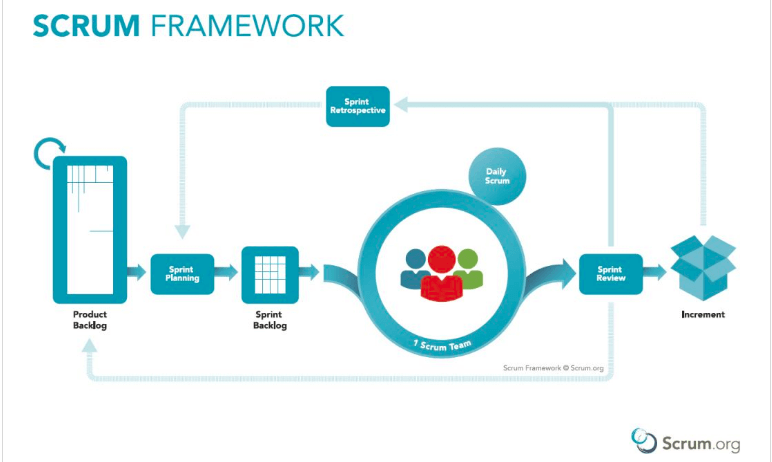
\includegraphics[scale=0.45]{img/scrum.png}
\end{center}
\legend{Fonte: Voitto (Scrum Framework, 2020).}
\end{figure}

Mais informações referentes ao framework Scrum pode ser encontrado em
\cite{scrum-guide}

\section{IMPLEMENTAÇÃO}

O objetivo em questão foi desenvolver um software para a área da saúde
(Hospitais) em que colaboradores tais como enfermeiros / médicos pudessem
cadastrar os pacientes diagnosticados com o COVID-19. A equipe foi estruturada
de forma a possibilitar maior integração e troca de informações para que o
software fosse desenvolvido não somente de forma técnica mas contendo todos os
requisitos importantes para que funcionasse corretamente registrando dados para
o acompanhamento dos casos.

Na tabela abaixo, mostramos um exemplo de como o time foi estruturado
considerando enfermeiros responsáveis por áreas diferentes dentro do hospital ,
para contribuir com informações sobre o cadastro de pacientes nos setores que
atuam. O desenvolvedor que assume as atividades de programação e escrita do
código, os analistas de sistemas fazendo o levantamento de requisitos e
mapeamento do processo , analista de teste acompanhando os resultados e
funcionamento do produto , o Product Owner e o Scrum Master.


\begin{figure}[htb]
\caption{\label{fig_Team_Master}Team Master}
\begin{center}
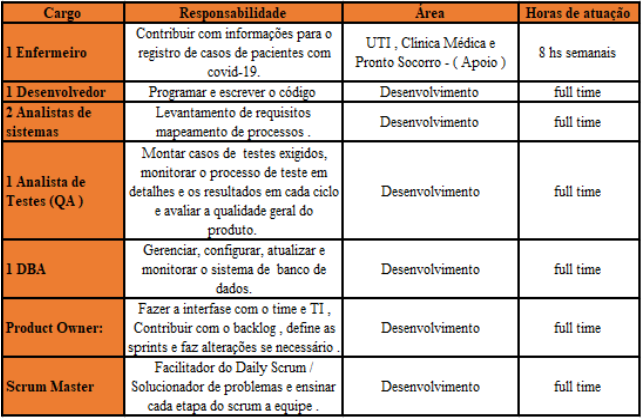
\includegraphics[scale=2.60]{img/team-master.png}
\end{center}
\legend{Fonte: Os autores}
\end{figure}

Agilidade adquirida com a implementação do Scrum contribuiu positivamente
para o desenvolvimento do software , respeitando a organização e o gerenciamento durante todo
o processo de criação até a entrega final do produto funcionando. Portanto conclui-se que, o
Scrum é um framework livre para organização de projetos podendo aliar-se com diversos
processos de desenvolvimento, já que suas regras não são imutáveis sendo possível
implementar apenas partes do Scrum e não o conjunto completo. E por ser simples e pequeno
funciona bem em qualquer contexto, projeto ou produto , porém precisa ser implementado
seguindo critérios de metodologias ágeis , considerando que o Scrum é um meio e não o fim,
capaz de transformar o gerenciamento e o desenvolvimento de softwares.

\section{ESTRUTURA DE DADOS}

A estrutura de dados utilizada neste programa foi lista encadeada simples
possui o campo e um específico que aponta para o próximo item da lista como
mostra a figura abaixo:

\begin{figure}[htb]
\caption{\label{fig_singly_linked_list}Lista Simplesmente Encadeada}
\begin{center}
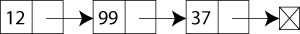
\includegraphics[scale=1.70]{img/singly_linked_list.png}
\end{center}
\legend{Fonte: Os autores}
\end{figure}

Nesta figura é apresentado uma lista de inteiros decimais para o campo dedos
que outro campo que aponta para o próximo item até chegar no final que aponta
normalmente para nulo.

A escolha desta estrutura de dados para armazenar o cadastro de pacientes foi a
simplicidade e facilidade de manipulação de dados, sendo apenas um pouco mais
complexa que um vetor, porém mais simples que estruturas como árvore binária, e
tendo a vantagem de ficar limitado apenas pela capacidade de hardware do
computador que irá executar o software. Uma base é um computador de porte
mediano pode armazenar informações de pacientes em memória cerca de 2361
pacientes diferentes sem problema algum de desempenho. E ocupando uma taxa
irrisória de memória de memória não volátil, porém de ponto negativo ocupa em
demasia memória volátil.

\section{FLUXO}

O fluxo de um programa é a parte crucial, é responsável por determinar para
qual parte do binário deve ser executada. C por ser uma linguagem estruturada
podemos saltar para blocos de código sem muita dificuldade executado da forma
que nos convém. Pelo programa ser feito por partes ou seja componentes as
condicionais podem simplesmente chamar o bloco de código correspondendo ao que
o usuário deseja. A figura abaixo explica o fluxo do software utilizando
fluxograma:

\begin{figure}[htb]
\caption{\label{fig_fluxo}fluxograma}
\begin{center}
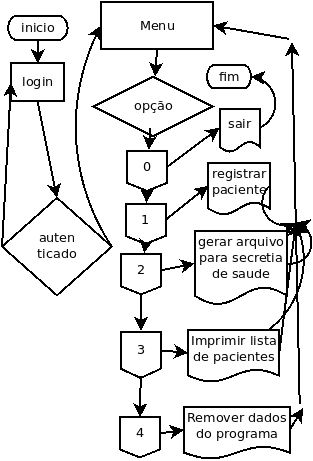
\includegraphics[scale=1.10]{img/fluxo.png}
\end{center}
\legend{Fonte: Os autores}
\end{figure}

\section{LEVANTAMENTO DE REQUISITOS}

Levantamento de Requisitos é uma estratégia de desenvolvimento de software que
funciona como ponto de partida para definir as etapas do desenvolvimento.
Normalmente é criado uma lista de requisitos obrigatórios no qual é usado a
sigla (RF) e para os requisitos obrigatórios e (RNF) para requisitos não
obrigatórios. Sendo descritos todos os requisitos que o sistema deve possuir.

Neste projeto foi levantado os seguintes requisitos obrigatórios:

\begin{itemize}
  \item{Informações referentes aos pacientes devem ser salvos em arquivo de
    texto puro}

  \item{Sistema de autenticação}

  \item{Verificar se o paciente está no grupo de risco possuindo mais que 65 anos
e comorbidades}

  \item{Gerar arquivo para secretaria da saúde com as informações de CEP e
idade dos pacientes no grupo de risco}

  \item{O software deve ser feito seguindo o paradigma procedural estruturado}
\end{itemize}

No qual serviu como fundação para o desenvolvimento do sistema e também foram
feitos a lista de requisitos não funcionais (RNF) para serem desenvolvidos caso houve
tempo no cronograma:

\begin{itemize}
  \item{biblioteca mínima para manipulação de datas brasileiras}
  \item{Evitar duplicatas de pacientes}
\end{itemize}

\section{COMPONETIZAÇÃO}

Componentização é um método de desenvolvimento muito que tem fortes
influências da filosofia Unix mais especificamente a frase Doug Mcllroy em 1968 “Faça com
que cada programa execute bem uma coisa. Para fazer um novo trabalho, crie de novo ao invés
de complicar programas antigos adicionando novos "recursos".”\cite{gancarz1995unix} . A mesma ideia pode ser
utilizada, dentro do mesmo programa, não a motivas de adicionar mais recursos a uma função
deixando ela complexa é melhor criar outra e então cada função faz apenas uma coisa e muito
bem feito.

Tratando o sistema como pequenas partes que foram um todo é possível diminuir a
complexidade do programa além de facilitar na distribuição de tarefas para cada
desenvolvedor.Uma dificuldade encontrada por seguir este método foi que linguagem de
programação escolhida não tem pleno suporte a programação orientada a Objetos e também um
dos requisitos do sistema foi seguir o paradigma estruturado.


\section{FERRAMENTAS}

\subsection{MinGW Compilador}

O MingW é projeto que oferece compiladores minimalista e eficazes para
compilação de código nativa para plataforma microsoft Windows sem a dependência de
quaisquer recursos oferecido pela Microsoft como a biblioteca de execução Microsoft C. A
escolha do compilador MingGW para plataforma Microsoft Windows foi escolhida pela
simples fato de suas licenças onde grande parte do código está sobre domínio público ou seja
livre de direitos autorais e outras sobre licenças permissivas com BSD,MIT/X11 e outras
licenças também muito permissivas.

\subsection{Gdb}

GDB abreviação de GNU Debugger é um programa que visa facilitar a depuração
de códigos escritos em C e outras linguagem é distribuído pela projeto GNU, uma de suas
funcionalidades é a possibilidade de “olhar” dentro de seu programa em tempo de execução e
saber em que ponto ocorreu o problema, além da opção de desmontagem ou seja você pode
visualizar o código de máquina que o compilador gera. Sendo de suma importância para
realização do trabalho por facilitar encontrar pontos de falha de segmentação, saber valores de
variáveis em tempo de execução, executar o programa linha a linha.

\subsection{Git}


Git é um software livre e open source amplamente utilizado para o versionamento
de softwares por ser simples e eficiente e muito fácil de aprender. Foi
desenvolvido inicialmente por Linus Torvalds para suprir a demanda de
contribuições em seu kernel conhecido como Linux. Em suma o git grava pontos na
história do programa podendo o usuário voltar para tais pontos a qualquer
momento, também pode criar novos ramos para o desenvolvimento, possuindo também
ferramentas de integração para tratamento de conflitos.

\subsection{Neovim}

Para o desenvolvimento de uma programa em C é necessário um editor de texto
puro, e a ferramenta escolhida para esta tarefa foi o Neovim que é um editor
hiperextensíveis baseado no vim com suporte nativo a LSP(Language Server
Protocol) no qual possibilidade verificar erros de sintaxe antes do processo de
compilação, além de possuir uma licença GPLv3 e MIT para seu código, podendo o
usuário da ferramenta ter uma melhor garantia de segurança e saber o'que o
software faz em seu computador.


\section{MANUAL DO USUÁRIO}

\subsection{Login}

Para que o usuário tenha acesso às funcionalidades do programa antes ele
precisa realizar a autenticação entrando com as informações de usuário e senha
sendo ambos “admin” ou seja no campo usuário preencher com “admin” sem aspas e
no campo senha preencher com “admin” sem aspas e após clicar na tecla enter.
Primeiro o usuário tem que pressionar a tecla “ 1 “ do teclado para escolher
fazer a autenticação e teclar enter como mostra a figura abaixo:

\begin{figure}[htb]
\caption{\label{fig_user_menu}Figura do Menu}
\begin{center}
  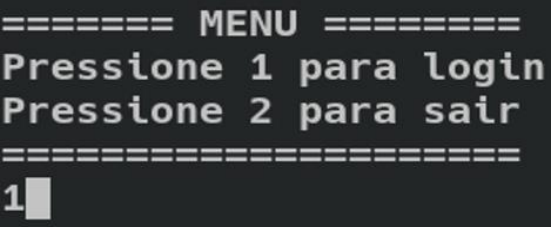
\includegraphics[scale=3.00]{img/user-menu.png}
\end{center}
\legend{Fonte: Os autores}
\end{figure}

Após a escolha da opção será redirecionado para o menu principal contendo as
seguintes funcionalidades como mostra a figura abaixo, podendo escolher entre
sair do programa, registrar novos pacientes, gerar arquivo para secretaria e
imprimir lista de pacientes como na figura abaixo:

\begin{figure}[htb]
\caption{\label{fig_user_menu_options}Figura do Menu de opções}
\begin{center}
  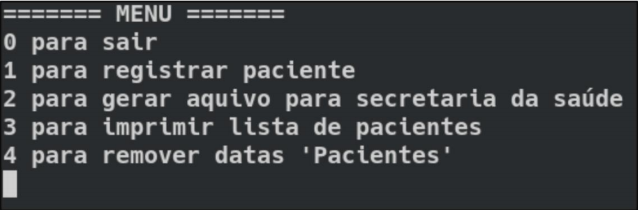
\includegraphics[scale=3.00]{img/login-options.png}
\end{center}
\legend{Fonte: Os autores}
\end{figure}

\subsection{Registro de pacientes}

Quando o usuário selecionar a opção número um para registrar um novo paciente
na lista, será pedido para ele entrar com as informação de nome, cpf, telefone,
endereço, data do diagnóstico, data de nascimento, email, cep e comorbidades,
em seguida automaticamente o programa ia criar uma arquivo em texto puro
contendo as informações do paciente junto a lista e caso algum paciente estiver
no grupo de risco será criado o arquivo para ser enviado a secretaria da saúde

\subsection{Imprimir lista de pacientes}

Quando o usuário selecionar a opção número três será exposto na tela a lista de
todos os pacientes já cadastrados. Na figura abaixo é mostrado um exemplo
fictício de como ficaria.


\begin{figure}[htb]
\caption{\label{fig_user_print_list}Figura da lista de pacientes cadastrados}
\begin{center}
  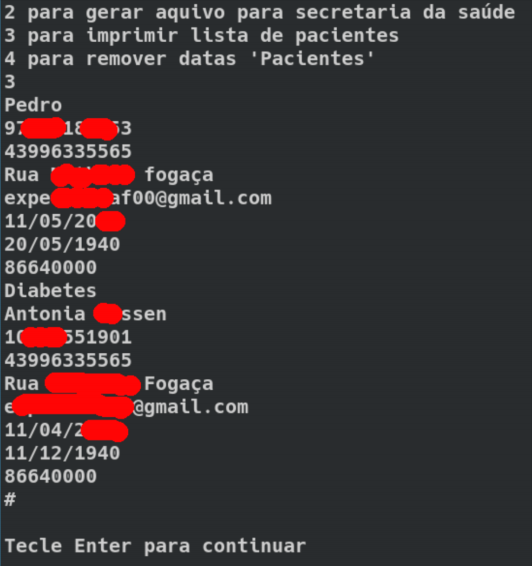
\includegraphics[scale=3.00]{img/user-print-list.png}
\end{center}
\legend{Fonte: Os autores}
\end{figure}

\subsection{Remover dados}

Quando o usuário pressionar o tecla número quatro o programa vai pedir uma
confirmação e caso o usuário digitar `S` maiúsculo o programa removerá os
arquivos `data.txt` que possui informações referentes a todos os usuários já
cadastrados, e o `secretaria.txt` que possui as informações de CEP e Idade dos
pacientes do grupo de risco

\section{CÓDIGO}

O código foi desenvolvido objetivando princípios de simplicidade e
funcionalidade única para manter um software simples, legível e fácil de manter
e ao mesmo tempo compatível com diversas plataformas e podendo ser executado em
quase todos os sistemas operacionais que possuem suporte a libc padrão. A fonte
do software pode ser encontrado hospedado no github na qual é a maior
plataforma de compartilhamento de código aberto do mundo, pode ser encontrado
no endereço: \url{https://github.com/PedroExpedito/trabalho} ou baixar o arquivo em
zip conforme as exigências da Unip em
\url{https://codeload.github.com/PedroExpedito/trabalho/zip/main.}

% ---
% Conclusão
% ---
\section{CONCLUSÃO}
O software desenvolvido neste projeto vai ajudar suprir a
necessidade dos hospitais de cadastrar grande quantidade de dados de pacientes,
realizando relatórios para enviar à secretaria da saúde municipal através de um
arquivo de texto, além disso irá apoiar nas tomadas de decisões durante todo o
processo de diagnóstico até o registro de casos, possibilitando a
intensificação de ações para prevenção e combate ao Covid-19. O cadastro será
feito de modo fácil e quase intuitivo, inclusive até pessoas com dificuldades
para utilizarem recursos tecnológicos poderão efetuar o cadastro sem
dificuldades.

Em parte técnica manteve um código legível de forma simplificada e
compreensível, com poucos erros de fácil manutenção e sem dependências que
dificultam a melhoria do software. Principal benefício de não possuir
dependências de software não livre, ou seja, o programa está sobre os direitos
do autor sem grandes interferências externas podendo ser alterado de maneira
rápida. 

A utilização do software ainda prevê otimizar processos longos de cadastros ,
reunindo apenas informações que sejam relevantes para melhor gerenciamento do
números de casos , apontando pacientes que são do grupo de risco e se possuem
patologias que elevam o grau de gravidade da doença , em quais regiões estes
pacientes estão localizados ,fazendo com que seja possível mapear bairros ,
cidades e estados com maior número de infectados e possibilita também entender
a capacidade mínima que os hospitais possuem para atendimento de pacientes com
Covid-19.

O diferencial deste produto não é apenas por ser um software livre,simples,
intuitivo , mas por ter sido construído com a finalidade de ser um facilitador
e uma solução tecnológica fundamental para sistematizar um serviço
imprescindível para a área da saúde, que em meio a todo esse caos vivenciado
nos dias atuais , o uso de recursos e ferramentas inteligentes e seguras podem
ser aliadas na gestão da saúde no brasil.

% ----------------------------------------------------------
% ELEMENTOS PÓS-TEXTUAIS
% ----------------------------------------------------------
\postextual

% ----------------------------------------------------------
% Referências bibliográficas
% ----------------------------------------------------------
\bibliography{abntex2-modelo-references.bib}


% ----------------------------------------------------------
% Glossário
% ----------------------------------------------------------
%
% Consulte o manual da classe abntex2 para orientações sobre o glossário.
%
%\glossary



% ----------------------------------------------------------
% Anexos
% ----------------------------------------------------------

% ---
% Inicia os anexos
% ---

%---------------------------------------------------------------------
% INDICE REMISSIVO
%---------------------------------------------------------------------

\phantompart

\printindex


\end{document}
